%% LaTeX_Thesis_Template.tex
% An unofficial LaTeX template for Cranfield theses.

%%
% This document is an example of the use of the unofficial "cranfieldthesis" 
% LaTeX style file.  I hope it's useful, and good like.

\documentclass[12pt]{book}

\usepackage[utf8]{inputenc}
% Use the custom "cranfieldthesis" LaTeX style file. 
\usepackage{cranfieldthesis}
\usepackage{xcolor}
\usepackage{graphicx}
\usepackage{float}

% By default, LaTeX uses a serif font - these are traditionally thought to be
% easier to read.   If you'd prefer sans-serif, please uncomment the 
% following line.
%\renewcommand{\familydefault}{\sfdefault}


% Example parameters for a typical taught MSc course
\title{Development of Physics or HPC Optimisation of a parallel 2D lattice Boltzmann solver using GPUs/CUDA}
\author{José Oliveira}
\date{August 2017}
\school{Aerospace, Transport and Manufacturing}
\course{Computational \& Software Techniques In Engineering}
\degree{MSc}
\academicyear{2016--2017}
\supervisor{Dr Irene Moulitsas}
\copyrightyear{2017}


\begin{document}


%% Front matter
%
% This is where we do the title page, etc.
%

\frontmatter

% Standard-Form Title Pages
\maketitle

% Abstract and Keywords
\begin{abstract}
    Type your abstract here.
    \section*{Keywords}
    Keyword 1; keyword 2; keyword 3.
\end{abstract}

% Table of Contents
\sstableofcontents

% List of Figures
\sslistoffigures

% List of Tables
\sslistoftables

% The list of abbreviations can't be automatically generated so you need to populate it yourself
\begin{listofabbreviations}
    \abbrev{CUDA}{Compute Unified Device Architecture}
    \abbrev{CFD}{Computational Fluid Dynamics}
    \abbrev{GPGPU}{General-purpose computing on graphics processing units}
\end{listofabbreviations}

% Acknowledgements
\chapter{Acknowledgements}
The author would like to thank \dots

%% Main Matter
%
% This is where we include the main thesis content.
%
\mainmatter

\chapter{Introduction}

\chapter{Literature review}
In this chapter, we will be taken into the broad field of the Lattice Boltzmann method using the CUDA platform. The topic of this thesis is associated with a number of different study areas, such as Computational Fluid Dynamics, Lattice Boltzmann method, High performance computing and GPGPU. We will then present an extensive literature review on these themes in the remaining of this chapter. Firstly, we will look into Computational Fluid Dynamics and the most commonly used approaches to it. Then we will be giving an overview on the Lattice Boltzmann method. Afterwards we will discuss how it is possible to employ parallelisation techniques in scientific computing. Finally we will review some previous works in this area.
\section{Computational Fluid Dynamics}
Computational Fluid Dynamics (CFD) comes from the need to model fluid flows and associated processes.
A wide range of applications come from studying CFD, notably:
\begin{itemize}
\item Aircraft design \cite{aircraft_cfd}
\item Solid particle erosion \cite{partic_erosion_cfd}
\item Wind flow simulation \cite{wind_flow_cfd}
\item Combustion chamber simulations \cite{combust_cfd}
\item Environmental and weather prediction \cite{weather_pred}
\item Automotive and motor sports \cite{america_cup,race_car_wing}
\end{itemize}

CFD can be used as a design and troubleshooting tool, as well as making the process dynamics easier to understand. It is used extensively by scientists and researchers, but it also has innumerable applications in the industry. CFD simulations is a viable tool for manufacturing because it eliminates expensive simulations.\par
 As such, it is the science of determining a solution to fluid flow through space and time \cite{cfd_present}. The models needed to calculate the fluid computations include:
\begin{itemize}
\item	Flow geometry
\item	Differential (Governing) equations – These describe the physics and chemistry of the flow
\item Boundary and initial conditions
\item	Discretization of the domain
\end{itemize}



\subsection{Macroscopic scale}
In this approach, the fluid can be seen as a collection of a huge number of particles. To solve these governing equations, one needs to apply conservation of energy, mass and momentum\cite{lbm_springer}. But since these equations are difficult, or even impossible to solve analytically, discrete schemes, boundary and initial conditions are used to convert these equations into a system of algebraic equations. These equations can then be solved until an appropriate solution is produced. {\color{red}NAVIERSTOKES}
\subsection{Microscopic scale}
If we consider the fluid to be represented by individual particles then we will fall under the microscopic approach. In this approach, there is no definition of temperature or viscosity and collision between particles needs to be considered. Thus one needs to solve the differential equation of Newton’s second law \cite{lbm_springer}. Hence, the location and velocity of each particle needs to be taken into account.
	\par We can easily see that this approach becomes unfeasible for normal fluid sizes as the number of equations needed to be solved grows to the order of billions (consider that one mole of water contains more than $6 \times 10^{23}$ molecules.


\section{Lattice Boltzmann Method}
The Lattice Boltzmann method (LBM) is a mesoscopic scale approach to CFD. It is used to describe a fluid based on probabilities using the Maxwell-Boltzmann equation in the fluid’s equilibrium state \cite{lbm_springer}. 
\par In this method, we do not consider the individual characteristics of each particle. By grouping particles together in a D2Q9 (nodes containing 9 particles for 2D problems - Fig \ref{fig:d2q9})  or in a D3Q19 (nodes containing 19 particles for 3D problems - Fig \ref{fig:d3q19}) model, we can analyse the behaviour of the particles collectively  \cite{lbm_springer}. 

\begin{figure}[H]
\centering
  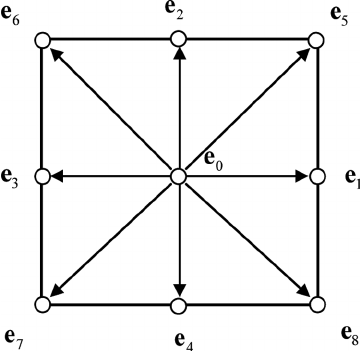
\includegraphics[width=0.3\linewidth]{Resources/Images/d2q9.png}
  \caption{2D LBM model using 9 particles. (D2Q9)}
  \label{fig:d2q9}
\end{figure}

\begin{figure}[H]
\centering
  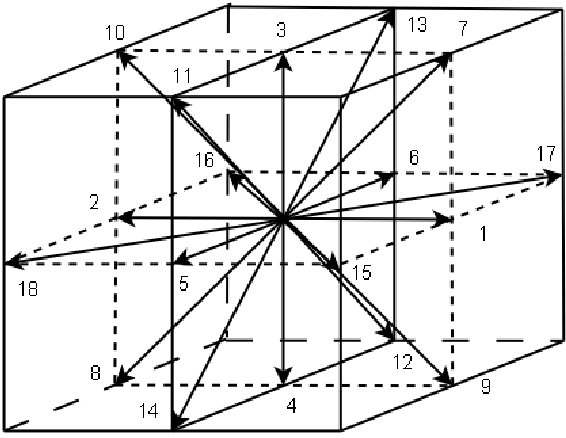
\includegraphics[width=0.3\linewidth]{Resources/Images/d3q19.png}
  \caption{3D LBM model using 19 particles. (D3Q19)}
  \label{fig:d3q19}
\end{figure}

\par
This way we can reap the advantages of both the macro and microscale approaches without the need of high end computers \cite{lbm_springer}. Since communications between nodes are very limited, LBM also offers the possibility of employing parallel computing to achieve the solution in even faster times.



\section{High Performance Computing}
As humanity evolves, so too does our desire for expanding previous unobtainable goals. As computer technology kept progressing further and further, we soon realised that some problems simply took too many resources to be completed. But what if instead of focusing on computational power we focused our efforts in splitting the workload? MOORE's LAW\par
High performance computing (HPC) comes from the harnessing of computer power to deliver a much higher performance that one could not obtain from a typical computer. To this end, we can talk of HPC as being a collection of computer resources, all of them working simulateously to achieve a solution of the same problem. DIFFERENT PARALLELISATION STRATEGIES FOR SPLITTING THE WORKLOAD EMERGE, DEPENDING ON THE UNDERLYING HARDWARE. Problems that could otherwise take weeks, months or even years can now be solved in minutes, hours or days under these powerful devices. 

\subsection{Distributed memory}
\subsection{Shared memory}

\subsection{GPGPU}

General Purpose computing on Graphical Processing Units stands for the use of Graphics Processing unit (GPU) to perform computations on applications normally performed by the CPU. One of the main advantages of using this approach is the amount of cores that a single GPU has. While a typical desktop CPU has up to 4 cores, a GPU can have thousands of cores, allowing users to take advantage of its massively parallel architecture. GPUS CAN NOW SOLVE PROBLEMS THAT WERE TRADITIONAL FOR CPU. GPU ARE CHEAPER AND ITS NOT POSSIBLE TO GET CPUS AS POWERFULL\par
	CUDA was then developed by NVIDIA SWITCH THE ORDER. CUDA code allows programmers to take advantage of GPUs by employing a unified shader pipeline under the familiar C language \cite{cuda_by_example}. Users were no longer required to have specific knowledge of OpenGL or DirectX and could now perform general computations (rather than graphic-specific computations) whilst benefiting from the massive computational powered offered by GPUs.  OPENCL

\section{Previous parallelisation works}
This thesis is a continuation of work that started some years ago in Cranfield University. As such, the work from the previous students needs to be analysed. \par
In 2014, Tamás Józsa and Máté Szőke, adapted two different inhouse C and C++ codes into one single C code unifying the advantages of each one of the two original codes \cite{jozsa_thesis,szoke_thesis}. Józsa then parallelised the critical parts of the C code using CUDA and ran tests on the Fermi GPU Cluster from Cranfield, achieving a three times speedup in general, with a peak of 15 times speedup \cite{jozsa_thesis}. \par
Szőke proposes a CPU APPROACH different parallelisation approach using Unified Parallel C, which is a Partitioned Global Address Space language\cite{szoke_thesis}. This means that it’s possible to use shared memory to compute the solution. However, the author verified that a local memory-based approach (like MPI) provided the best results. He also compared the results obtained with the ones obtained by Józsa on the CUDA approach. They found that to achieve the same speed-up as that of a single GPU card, one needs an entire workstation (16 threads in the case of Astral) \cite{szoke_thesis}.\par
In 2015, Ádám Koleszár continued the work and further optimised the parallel version of the LBM method using CUDA \cite{koleszar_thesis}. He did an excellent job, resulting in a 10 times faster execution than the previous 2D parallel solver, which means that his new optimised code was 30 times faster than the original, in-house, serial solver.\par
Finally, in 2016, Maciej Kubat proposed a new version of the LBM solver.Firstly he converts the 2D parallel solver to a 3D parallel solver which entailed a major reengineering of the code, from data containers to logic cycles \cite{maciej_thesis}. After first trying for a direct adaptation, he found that his code was too slow to produce meaningful solutions. After optimising his own code he was able to reach an almost one hundred times speedup.
However, Kubat states that a lot can be done to improve his code, from boundary conditions to code readability and maintainability. 

\chapter{Conclusions}

%% Back matter
%
% This is where we include appendices and references

\appendix

\bibliography{AllBib}{}
\bibliographystyle{plain}
\end{document}